% TODO (lots of stuff!!!!)
%
% -- Write presubmission inquiry (Nature, Science, PLOS Biology).
%
% -- People to Contact:
% ---- The guys from Haldane's Sieve
% ---- Jonathan Eisein
% ---- Carl Boettinger
% ---- Jarrett Byrnes
% ---- Twitter call (?)
%
% -- Journals to contact:
% ---- Evolution
% ---- Journal of Evolutionary Biology
% ---- British Ecological Society

\documentclass[letterpaper,twocolumn,superscriptaddress,showkeys]{revtex4}
\usepackage[utf8]{inputenc}
\usepackage{color,dcolumn,graphicx,hyperref}
\hypersetup
{
    colorlinks = true, linkcolor = blue, citecolor = blue, urlcolor = blue,
}

\begin{document}

\title{Preprints in Ecology \& Evolution}
% Alternative title: arXiv or die!

\author{Philippe Desjardins-Proulx}
\email[E-mail: ]{philippe.d.proulx@gmail.com}
\affiliation{Theoretical Ecosystem Ecology laboratory, Universit\'e du Qu\'ebec \`a Rimouski, Canada.}
\affiliation{Quebec Center for Biodiversity Science, McGill University, Canada.}
\affiliation{D\'epartement des sciences biologiques, Universit\'e du Qu\'ebec \`a Montr\'eal, Canada.}

\author{Ethan P. White}
\affiliation{Departement of Bology, Utah State University, United-States of America.}

\author{Timoth\'ee Poisot}
\affiliation{Theoretical Ecosystem Ecology laboratory, Universit\'e du Qu\'ebec \`a Rimouski, Canada.}
\affiliation{Quebec Center for Biodiversity Science, McGill University, Canada.}
\affiliation{International Network for Next-Generation Ecology.}

\author{Dominique Gravel}
\affiliation{Theoretical Ecosystem Ecology laboratory, Universit\'e du Qu\'ebec \`a Rimouski, Canada.}
\affiliation{Quebec Center for Biodiversity Science, McGill University, Canada.}

\keywords{Publishing; arXiv; Green Open Access.}

\begin{abstract}

...
 
\end{abstract}

\maketitle

\section{The case for open preprints}

% Main arguments:

%% Take a look at arXiv usage and how its impact (Tim's suggestion)
% I know some papers were published on the impact of articles on arXiv
% in high-particle physics.

%% Speed up science.

%% Essentially an open equivalent to sharing preprints between colleagues.

\begin{figure}[ht!]

\centering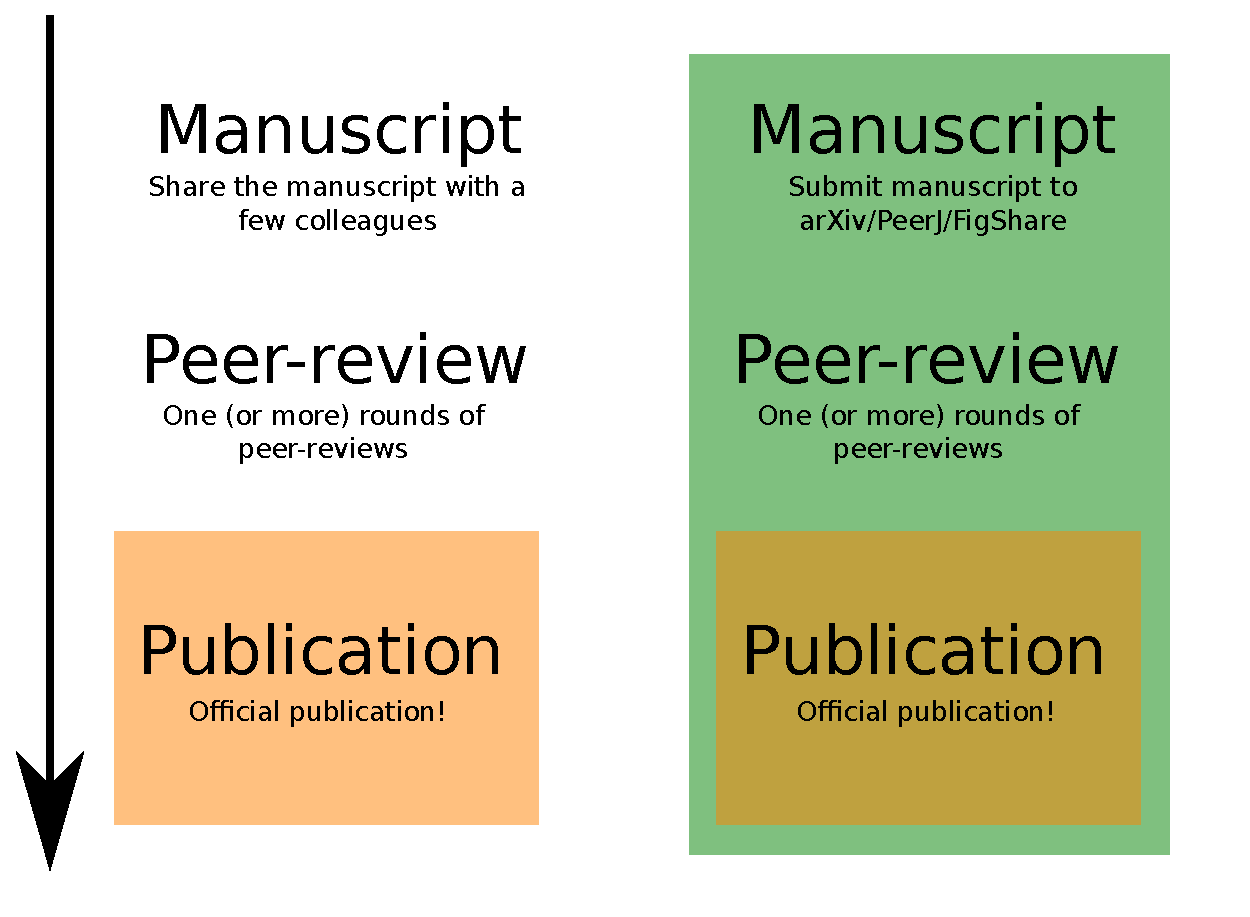
\includegraphics[width=0.50\textwidth]{map.pdf}
\caption
{
    Since the time between submission and
}
\label{fig:map}

\end{figure}

%% Establish priority in a fair way:

% I think this argument is important since biologists often think people will
% "steal" their ideas, while physicists and mathematicians see arXiv as a way to
% establish priority.

\section{Preprints, Ecology \& Evolution}

While the practice is still rare, preprints are becoming more common in
biological sciences, which is experiencing faster growth in arXiv submission
than any other fields \cite{cal12}. Also, most scientific journals are
preprint-friendly: Nature, PLOS, BMC, PNAS, Science (mostly), and all the
journals from Elsevier and Springer. Very recently, the Ecological Society of
America recently changed its policy to allow public preprints (REF). In our
field, very few scientific publications will not consider a manuscript
submitted to arXiv. Many ecology \& evolution journals adopt a ``by default''
hostile attitude towards preprints, mostly due to the lack of clear policy of
the publishers. As an example, Wiley-Blackwell, which publishes some of the
leading journal in the field (a quick lsit), has no official policy on the
subject.

% A table?
%% Journal | Publisher | ISI rank | Official policy ?

\section{Current offer}

% Short paragraphs on the current open preprint repositories.

\subsection{arXiv}

arXiv (\href{http://arxiv.org/}{http://arxiv.org/})

arXiv is funded by a network of universities.

\subsection{Figshare}

Figshare (\href{http://figshare.com/}{http://figshare.com/})

All figshare content (article, figures, datasets) have a unique digital object
identifier (DOI) like any journal article.

\subsection{PeerJ}

% Ethan P. White's section

\subsection{F1000Research}

% Not really the same, but worth mentionning.

\section{Conclusion}

% A short paragraph to conclude.

Responding to the rumour that their refused manuscripts submitted to arXiv,
Nature responded that ``Nature never wishes to stand in the way of communication
between researchers. We seek rather to add value for authors and the community
at large in our peer review, selection and editing'' \cite{nat05}.

\newpage
\bibliography{refs}
\bibliographystyle{plain}

\end{document}

